\chapter{Ответы на вопросы}

\section{Элементы языка}

Элементами языка являются атомы и точечные пары.

\textbf{Атомы} представляю из себя:
\begin{enumerate}
	\item Символы --- синтаксически представляется как набор букв и цифр, начинающийся с буквы.
	\item Специальные символы --- \{T, Nil\}.
	\item Самоопределимые атомы --- натуральные, дробные и вещественные числа, а также строки, заключенные в двойные апострофы. 
	% Их значение переопределить нельзя.
\end{enumerate}

Атомы обычно выглядит как последовательность букв или цифр.

Примеры атомов:
\begin{lstlisting}
	B
	CAT
	Я123Атом
	ВотЭтоТожеАтом
	123
	T
	Nil
	2/3
	"abc"
\end{lstlisting}

\textbf{Точечная пара} --- (A . B). Строится с помощью бинарных узлов.   

\begin{lstlisting}
	Точечная  пара ::= (<атом>.<атом>) |
	(<атом>.<точечная пара>) |
	(<точечная пара>.<атом>) |
	(<точечная пара>.<точечная пара>)	
\end{lstlisting}

Пример точечной пары:
\begin{lstlisting}
	(A . (B . (C . (D . Nil))))
\end{lstlisting}
Облегченная форма записи:
\begin{lstlisting}
	(A B C D)
\end{lstlisting}

\begin{figure}[ht!]
	\centering{
		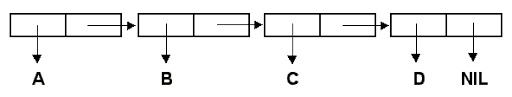
\includegraphics[width=0.9\textwidth]{src/img1}
		\caption{Представление в памяти (A B C D).} }
\end{figure}

\textbf{Представление в памяти:}

\begin{enumerate}
	\item \textbf{(A . B)}
	\begin{figure}[ht!]
		\centering{
			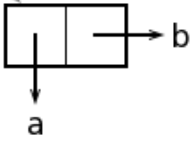
\includegraphics[width=0.2\textwidth]{src/img3}
			\caption{Представление в памяти (A . B).} }
	\end{figure}
	\item \textbf{(A B)} --- экономия памяти, но проблема при рекурсивной обработке (т.к. не сможем идентифицировать конец, как Nil)
	\begin{figure}[ht!]
		\centering{
			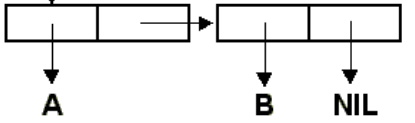
\includegraphics[width=0.5\textwidth]{src/img2}
			\caption{Представление в памяти (A B).} }
	\end{figure}
\end{enumerate}

\begin{lstlisting}
	S-выражение ::= <атом> | <точечная пара>
\end{lstlisting}

Список является частым случаем S-выражения.

S-выражение представлено 

\begin{figure}[ht!]
	\centering{
		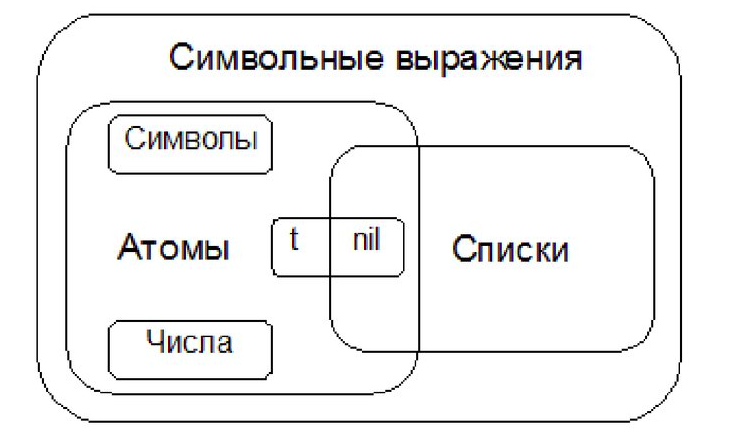
\includegraphics[width=0.5\textwidth]{src/img4}
		\caption{S-выражение} }
\end{figure}

\textbf{Список} --- динамическая структура данных, которая может быть
пустой или непустой. Если она не пустая, то состоит из двух элементов:

1. Головы --- любая структура.

2. Хвоста --- список.

Список представляет из себя заключенную в скобки
последовательность из атомов, разделенных пробелами, или списков.
Любой список является программой - его нужно вычислять.

Примеры списков:
\begin{lstlisting}
	(A B C)
	(1 2 3)
	((A B) (C D))
\end{lstlisting}

\textbf{Синтаксис}

Lisp является регистронезависимым языком. 

Универсальным разделителем, между атомами, является пробел. В начальных версиях была предложена запятая, но она не прижилась.

Наличие скобок является признаком структуры - списка или точечной пары.
% Ограничитель - круглые скобки.

\textbf{Специальные символы:}
\begin{enumerate}
	\item \textbf{T} --- Константа. обозначает логическое значение "истина". Истинным значением является все, что отличное от Nil.
	\item \textbf{Nil} --- "ложь". Также обозначает пустой список. Записи nil и () эквивалентны. Являются синтаксисом пустого списка
\end{enumerate}

Любая структура заключается в круглые скобки.

(A . B) - точечная пара.

(A) - список из одного элемента.

() или Nil - пустой список.

Одноуровневый список:
\begin{lstlisting}
	(A B C D)
\end{lstlisting}

Структурированный список:
\begin{lstlisting}
	(A (B C) (D E))
\end{lstlisting}

\textbf{Как воспринимается символ апостроф}

Символ апостроф --- синоним quote.

\textbf{quote} --- блокирует вычисление своего аргумента.
В качестве своего значения выдаёт сам аргумент, не вычисляя его.
Перед константами - числами и атомами T, Nil можно не ставить апостроф.
% т.к. значением любой константы является она сама.

Пример использования quote:
\begin{lstlisting}
	(quote (car (A B C))) => (car (A B C))
\end{lstlisting}

% \begin{lstlisting}
	% 	(quote (EVAL (ATOM B))) => (EVAL (ATOM B))
	% \end{lstlisting}

Вычисление начинается с внешней функции quote, которая возвращает аргумент в неизмененном виде.

\section{Базис лиспа}

\textbf{Базис} --- минимальный набор средств для решения любой задачи.

Базис:

1) атомы и бинарные узлы;

2) atom, eq, cons, car, cdr, cond, quote, eval.

atom проверяет, является ли объект, переданный в качестве аргумента, атомом.

\begin{lstlisting}[language=Lisp]
	(atom 'a) ;; t
	(atom '(a b c)) ;; nil
\end{lstlisting}

eq проверяет идентичность двух символов.
\begin{lstlisting}[language=Lisp]
	(eq 'a 'b) ;; nil
	(eq 'a 'a) ;; t
\end{lstlisting}

cond --- сокращение от англ. condition --– условие. 
Не имеет фиксированного количества аргументов.
Каждый аргумент --- это список, голова которого рассматривается как условие, 
и если оно истинно, то результатом будет хвост рассматриваемого списка.

\begin{lstlisting}
	(cond ((eq 'A 'B) 'are_equal)
	(T 'not_equal)) ;; NOT_EQUAL
\end{lstlisting}

eval - выполняет двойное вычисление своего аргумента.

\begin{lstlisting}
	(eval (cons (quote car) (quote ('(A B))))) => A
	|---------(car '(A B))---------|
	
\end{lstlisting}


\textbf{Функции car и cdr}

car и cdr - базовые функции доступа к данным. 

\textbf{car} --- принимает точечную пару или список и возвращает голову (первый элемент).

\textbf{cdr} --- принимает точечную пару или список и возвращает хвост (все элементы, кроме первого).

\textbf{Отличие list и cons}

cons --- имеет фиксированное количество аргументов (два). 
В случае, когда аргументами являются атомы создает точечную пару.
В случает, когда первый аргумент атом а второй список, атом становится головой,
а второй аргумент (список) становится хвостом. 
\begin{lstlisting}[language=Lisp]
	(cons 'a 'b) 		 ;; (A . B)
	(cons 'a '(a b c)) 	 ;; (A A B C)
	(cons '(a c) '(b d)) ;;((A C) B D)
	(cons 'a 'v 'd)  	 ;; Error (invalid number of arguments: 3)
\end{lstlisting}

\begin{figure}[ht!]
	\centering{
		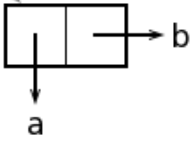
\includegraphics[width=0.25\textwidth]{src/img3.png}
		\caption{Результат cons.} }
\end{figure}

list --- не имеет фиксированное количество аргументов. 
Создает список, у которого голова --- это первый аргумент,
хвост --- все остальные аргументы.
\begin{lstlisting}[language=Lisp]
	(list 'a 'b) 				;; (A B)
	(list 'a 'b 'v '(c d) 'd) 	;; (A B V (C D) D)
\end{lstlisting}

\begin{figure}[ht!]
	\centering{
		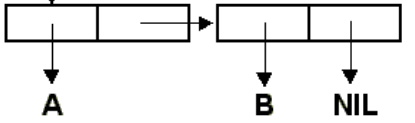
\includegraphics[width=0.5\textwidth]{src/img2.png}
		\caption{Результат list.} }
\end{figure}

\textbf{cons} --- имеет фиксированное число аргументов и более экономный по памяти.

\textbf{Ядро} --- основные действия, которые наиболее часто используются. Ядро шире, чем базис.
